\documentclass[notes,blackandwhite,mathsans,usenames,dvipsnames]{beamer}

\usepackage{amsmath}
\usepackage{amssymb}
\usepackage{graphicx}
\usepackage{fancybox}
\usepackage{booktabs}
\usepackage{multirow,pxfonts}
\usepackage{cmbright}
\usepackage{xcolor}
\usepackage{color}
\usepackage{enumitem}
\usepackage{animate}
\usepackage{changepage}

\usepackage[T1]{fontenc}
\fontencoding{T1}  
\usepackage[utf8]{inputenc}


\usefonttheme{default}
\setbeamercovered{invisible}
\beamertemplatenavigationsymbolsempty

\makeatletter
\setbeamertemplate{footline}
{
  \leavevmode
  \hbox{
  \begin{beamercolorbox}[wd=0.97\paperwidth,ht=2.25ex,dp=2ex,right]{}
{\color{mcxs2} \insertframenumber{} / \inserttotalframenumber}
  \end{beamercolorbox}}%
}


\definecolor{mcxs1}{HTML}{05386B}
\definecolor{mcxs2}{HTML}{379683}
\definecolor{mcxs3}{HTML}{5CDB95}
\definecolor{mcxs4}{HTML}{8EE4AF}
\definecolor{mcxs5}{HTML}{EDF5E1}
\setbeamercolor{frametitle}{fg=mcxs2}
\AtBeginDocument{\color{mcxs1}}
\setbeamertemplate{itemize item}[triangle]


\begin{document}
%\fontfamily{pag}\selectfont
%\setbeamerfont{title}{family=\fontfamily{pag}\selectfont}
%\setbeamerfont{frametitle}{family=\fontfamily{pag}\selectfont}
%\setbeamerfont{framesubtitle}{family=\fontfamily{pag}\selectfont}







{\setbeamercolor{background canvas}{bg=mcxs5}
\begin{frame}

\vspace{1cm}
\begin{tabular}{rl}
&\textbf{\LARGE\color{mcxs2} Macroeconometrics}\\[8ex]
\textbf{\Large Lecture 19}&\textbf{\Large\color{mcxs3}Modeling trend inflation}\\[19ex]
&\textbf{Tomasz Wo\'zniak}\\[1ex]
&{\small\color{mcxs3} Department of Economics}\\
&{\small\color{mcxs3}University of Melbourne}
\end{tabular}

\end{frame}
}




{\setbeamercolor{background canvas}{bg=mcxs5}
\begin{frame}

\vspace{1cm}\textbf{\color{mcxs2}A first look at the data... no one said it's gonna be easy!}

\bigskip\textbf{\color{mcxs2}UC models for Australian CPI inflation}

\bigskip\textbf{\color{mcxs2}UC model for Australian CPI prices}

\bigskip\textbf{\color{mcxs1}UC model for Australian Real GDP}

%\vspace{1cm} Useful readings: \footnotesize
%
%\smallskip{\color{mcxs2}Stock \& Watson (2016) Core Inflation and Trend Inflation, Review of Economics and Statistics}

\normalsize
\vspace{1cm} Materials: \scriptsize

\smallskip{\color{mcxs2}A zip file} \texttt{L19 mcxs.zip} {\color{mcxs2}for the reproduction of the results}

\end{frame}
}



{\setbeamercolor{background canvas}{bg=mcxs5}
\begin{frame}

\bigskip\textbf{\color{mcxs1}Objectives.}
\begin{itemize}[label=$\blacktriangleright$]
\item {\color{mcxs1}To familiarise with the parameters, trend, and cycle estimates}
\item {\color{mcxs1}To investigate the definition of the trend via the model specification}
\item {\color{mcxs1}To document the prior dependence of the results}
\end{itemize}

\bigskip\textbf{\color{mcxs2}Learning outcomes.}
\begin{itemize}[label=$\blacktriangleright$]
\item {\color{mcxs2}Documenting the persistence properties of the data}
\item {\color{mcxs2}Visualising the trend and cycle}
\item {\color{mcxs2}Performing prior robustness checks}
\end{itemize}

\end{frame}
}




{\setbeamercolor{background canvas}{bg=mcxs5}
\begin{frame}

\begin{adjustwidth}{-0.5cm}{0cm}
\vspace{8.3cm}
\textbf{{\color{mcxs2}A first look at the data...} {\color{mcxs3}no one said it's gonna be easy!}}
\end{adjustwidth}

\end{frame}
}



\begin{frame}{Consumer Price Index in Australia}

\centering
\includegraphics[scale=0.55, trim=2cm 1cm 2cm 0cm]{results/data-cpi-downloaded.pdf}

\bigskip\small{\color{mcxs2}
Quarterly data from 1949Q3 to 2022Q1 ($T=295$)\\ 
Downloaded from the ABS using }\\ \texttt{readabs::read\_abs(series\_id = "A2325846C")}

\end{frame}




\begin{frame}{Consumer Price Index in Australia}

\centering
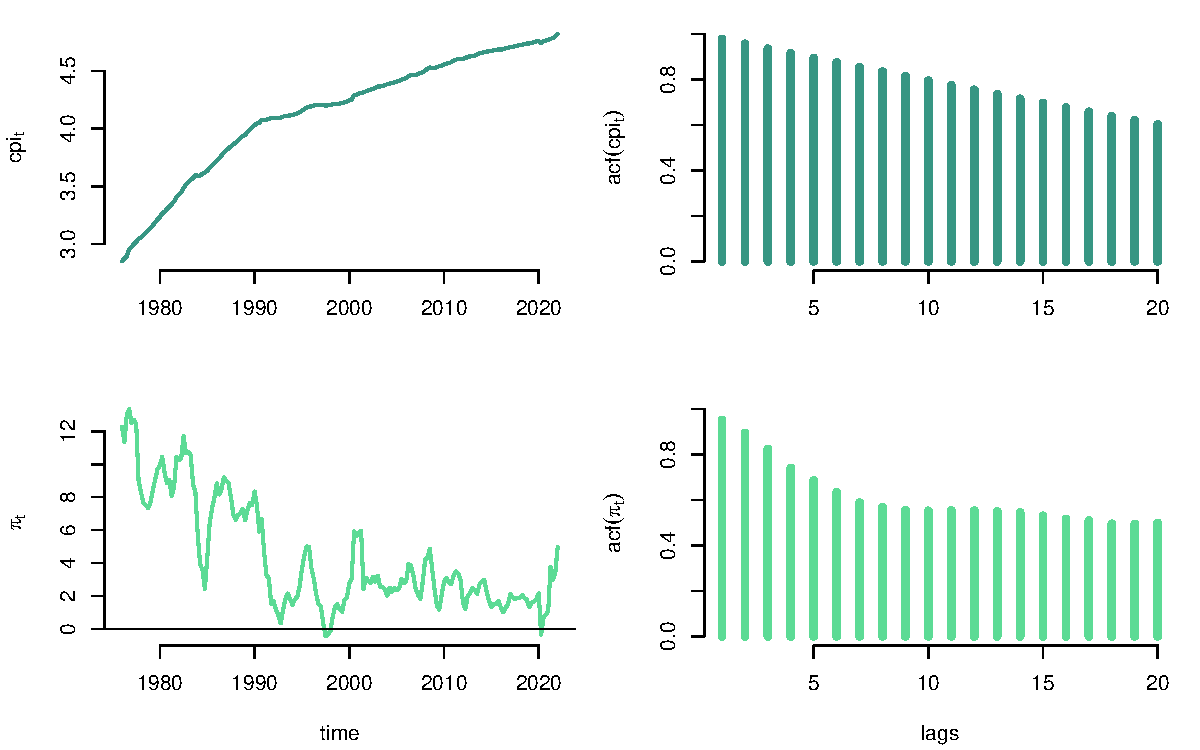
\includegraphics[scale=0.55, trim=2cm 0.5cm 2cm 0cm]{results/data-cpi.pdf}

\bigskip\small{\color{mcxs2}
$cpi_t= log(CPI_t) \qquad {\color{mcxs3}\pi_t = 100(cpi_t - cpi_{t-4})}$\\[0.5ex]
Quarterly data from 1976Q1 to 2022Q1 ($T=185$)}

\end{frame}


\begin{frame}{Consumer Price Index in Australia}

\begin{center}
\textbf{Integration order verification}\\
{\color{mcxs2}Quarterly data from 1976Q1 to 2022Q1}

\smallskip
\begin{tabular}{ccccc}
\toprule
 & deterministic & lag& & \\
variable& terms & order & $t_{ADF}$ & p-value\\
\midrule
$cpi_t$ & trend, constant & 24 & -2.776 & 0.252 \\
$cpi_t$ & constant & 24 & -0.922 & 0.714 \\[0.5ex]
\midrule
$\pi_t$ & constant & 23 & -2.324 & 0.193 \\
$\pi_t$ &  none & 23 & -2.29 & 0.023 \\[0.5ex]
\midrule
$\Delta \pi_t$ & none & 22 & -2.868 & <0.01 \\[0.5ex]
\bottomrule
\end{tabular}

\smallskip \small{\color{mcxs2}Computations performed using} \texttt{fUnitRoots::adfTest}
\end{center}
\end{frame}








{\setbeamercolor{background canvas}{bg=mcxs5}
\begin{frame}

\begin{adjustwidth}{-0.5cm}{0cm}
\vspace{8.3cm}\Large
\textbf{{\color{mcxs3}UC models for} {\color{mcxs1}Australian CPI inflation}}
\end{adjustwidth}

\end{frame}
}









\begin{frame}{Australian CPI inflation}

\bigskip\textbf{UC-AR(p) model with hierarchical prior for variances.}
\begin{align*}
y_t &= \tau_t + \epsilon_t\\[1ex]
\tau_t &= \mu + \tau_{t-1} + \eta_t\\[1ex]
\epsilon_t &= \alpha_1\epsilon_{t-1} + \dots + \alpha_p\epsilon_{t-p} +  e_t\\[2ex]
\begin{bmatrix}\eta_t \\ e_t\end{bmatrix}&\bigg|Y_{t-1} \sim ii\mathcal{N}\left(\mathbf{0}_2, \begin{bmatrix}\sigma_\eta^2 & 0 \\  & \sigma_e^2\end{bmatrix} \right)
\end{align*}

\smallskip\textbf{Prior hyper-parameters.}
\begin{align*}
\underline\alpha &= \mathbf{0}_p,  \qquad\underline{V}_\alpha = \kappa_1I_p, \qquad\kappa_1=1, \qquad \alpha\in A\text{  -- not imposed}\\
\underline\beta &= \mathbf{0}_2,  \qquad\underline{V}_\beta = \kappa_2I_2, \qquad\kappa_2=1\\
\underline\nu &=3, \qquad s= 0.00346, \qquad a= 1
\end{align*}

%$\sigma^2_\eta / \sigma^2_e$ {\color{mcxs2}-- signal-to-noise ratio}

{\color{mcxs2}Estimation via Gibbs sampler as presented in Lectures 17 \& 18}

\end{frame}







\begin{frame}{Australian CPI inflation}

\small
\begin{center}
\textbf{Estimation results from UC-AR(p) models:} {\color{mcxs2}$\pi_t$ 1976Q1--2022Q1}

\footnotesize\smallskip\begin{tabular}{ccccccccc}
\toprule
$p$ & $\alpha_1$ & $\alpha_2$ & $\alpha_3$ & $\alpha_4$ & $\alpha_5$& \% s  & $\mu$  & $\sigma^2_\eta / \sigma^2_e$\\
\midrule
1 & 0.893 &  &  &  &  & 95.9 & -0.011 & 2.009 \\ 
   & 0.091 &  &  &  &  &  & 0.055 &  \\ [1ex]
  2 & 1.221 & -0.346 &  &  &  & 98.4 & -0.015 & 2.288 \\ 
   & 0.203 & 0.213 &  &  &  &  & 0.054 &  \\ [1ex]
  3 & 1.092 & -0.003 & -0.267 &  &  & 99.8 & -0.018 & 1.398 \\ 
   & 0.131 & 0.181 & 0.111 &  &  &  & 0.048 &  \\ [1ex]
  4 & 0.838 & 0.158 & 0.101 & -0.395 &  & 100 & -0.022 & 0.750 \\ 
   & 0.108 & 0.130 & 0.130 & 0.115 &  &  & 0.039 &  \\ [1ex]
  5 & 1.025 & 0.089 & 0.037 & -0.624 & 0.330 & 99.2 & -0.026 & 0.382 \\ 
   & 0.095 & 0.119 & 0.119 & 0.128 & 0.100 &  & 0.033 &  \\ [1ex]
\bottomrule
\end{tabular}

\smallskip 
\% s -- fraction of posterior draws for which stationarity condition holds\\
$\sigma^2_\eta / \sigma^2_e$ -- signal-to-noise ratio
\end{center}

\end{frame}





\begin{frame}{Australian CPI inflation}

\small
\centering
\smallskip\textbf{Estimated trend and cycle from UC-AR(4)}

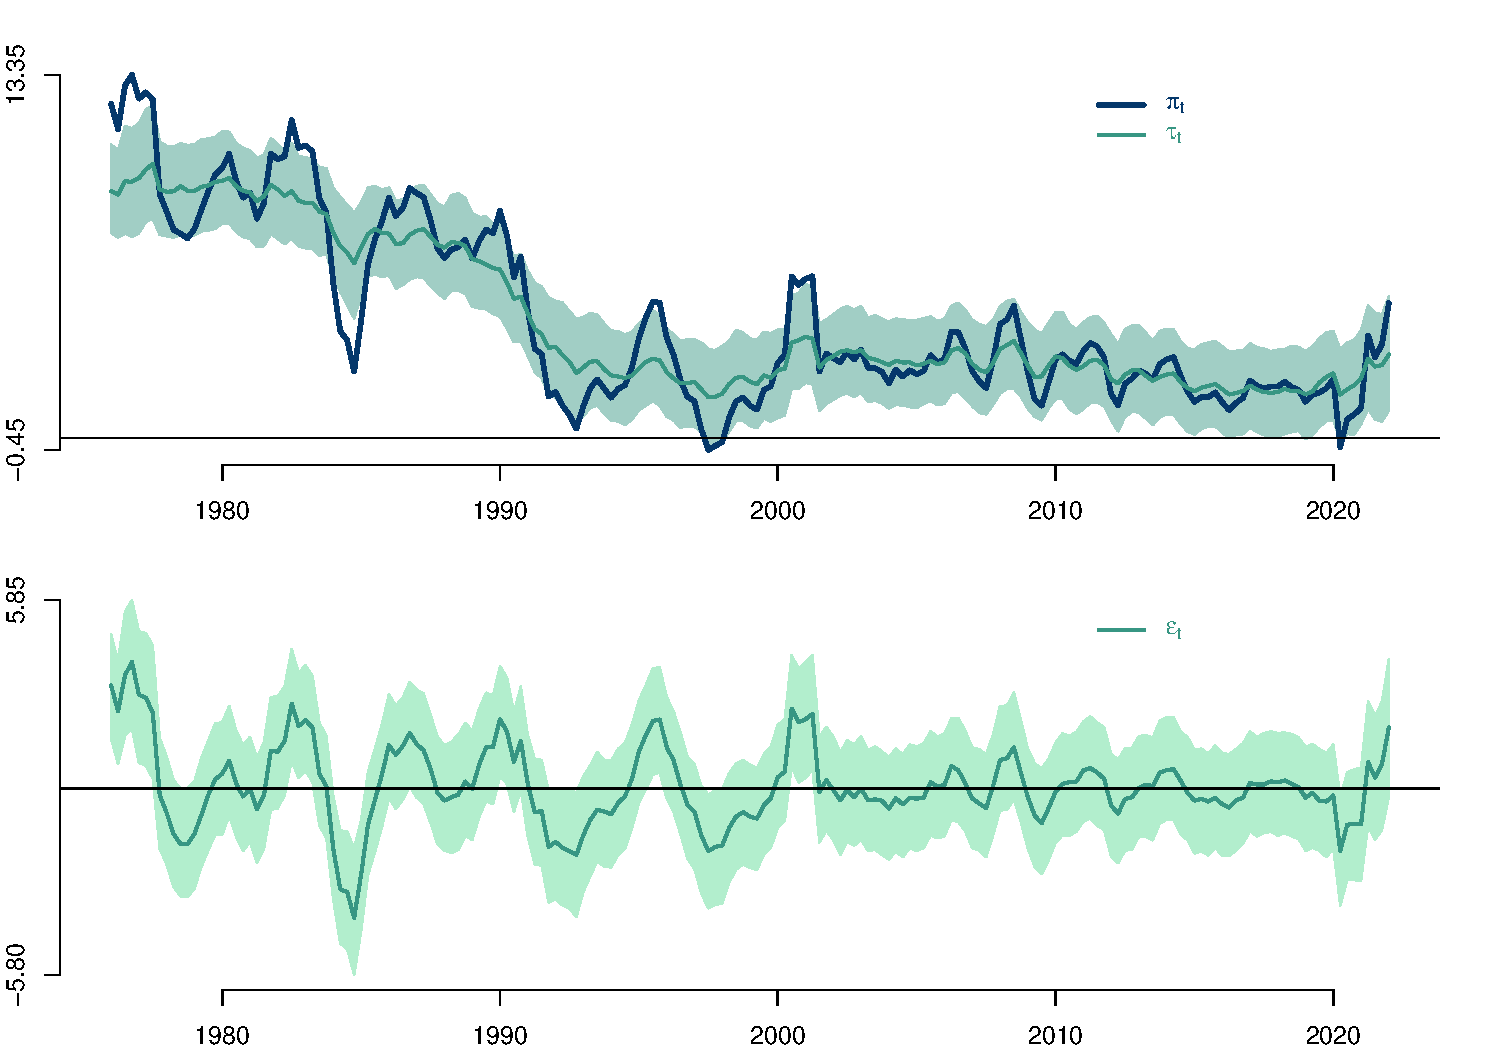
\includegraphics[scale=0.4, trim=2cm 0.5cm 2cm 0cm]{results/pi-sigma-uc-ar4.pdf}

\end{frame}









\begin{frame}{Australian CPI inflation}

\bigskip\textbf{UC-AR(p) with hierarchical prior and correlated shocks.}
\begin{align*}
y_t &= \tau_t + \epsilon_t\\[1ex]
\tau_t &= \mu + \tau_{t-1} + \eta_t\\[1ex]
\epsilon_t &= \alpha_1\epsilon_{t-1} + \dots + \alpha_p\epsilon_{t-p} +  e_t\\[2ex]
\begin{bmatrix}\eta_t \\ e_t\end{bmatrix}&\bigg|Y_{t-1} \sim ii\mathcal{N}\left(\mathbf{0}_2, \begin{bmatrix}\sigma_\eta^2 & \rho\sigma_\eta\sigma_e \\  & \sigma_e^2\end{bmatrix} \right)
\end{align*}

\smallskip\textbf{Prior hyper-parameters.}
\begin{align*}
\underline\alpha &= \mathbf{0}_p,  \qquad\underline{V}_\alpha = \kappa_1I_p, \qquad\kappa_1=1, \qquad \alpha\in A\text{  -- not imposed}\\
\underline\beta &= \mathbf{0}_3,  \qquad\underline{V}_\beta = \kappa_2I_3, \qquad\kappa_2=1\\
\underline\nu &=3, \qquad s= 0.00346 , \qquad a= 1
\end{align*}

\end{frame}





\begin{frame}{Australian CPI inflation}

\small
\begin{adjustwidth}{-0.5cm}{0cm}
\begin{center}
\textbf{Estimation results from UC-AR(p) models:} {\color{mcxs2}$\pi_t$ 1976Q1--2022Q1}

\footnotesize\smallskip\begin{tabular}{cccccccccc}
\toprule
$p$ & $\alpha_1$ & $\alpha_2$ & $\alpha_3$ & $\alpha_4$ & $\alpha_5$& \% s  & $\mu$ & $\rho$  & $\sigma^2_\eta / \sigma^2_e$\\
\midrule
2 & 1.240 & -0.374 &  &  &  & 97/7 & -0.011 & 0.056 & 4.693 \\ 
   & 0.266 & 0.262 &  &  &  &  & 0.079 & 0.053 &  \\ [1ex]
  3 & 1.038 & -0.025 & -0.246 &  &  & 99.6 & -0.014 & 0.079 & 7.583 \\ 
   & 0.313 & 0.244 & 0.212 &  &  &  & 0.066 & 0.060 &  \\ [1ex]
  4 & 0.828 & 0.139 & 0.105 & -0.398 &  & 99.8 & -0.020 & 0.132 & 2.380 \\ 
   & 0.179 & 0.196 & 0.187 & 0.165 &  &  & 0.057 & 0.069 &  \\ [1ex]
  5 & 1.013 & 0.094 & 0.054 & -0.664 & 0.331 & 99.1 & -0.023 & 0.102 & 1.184 \\ 
   & 0.132 & 0.149 & 0.148 & 0.154 & 0.126 &  & 0.058 & 0.064 &  \\ [1ex]
\bottomrule
\end{tabular}

\smallskip 
\% s -- fraction of posterior draws for which stationarity condition holds\\
$\sigma^2_\eta / \sigma^2_e$ -- signal-to-noise ratio
\end{center}
\end{adjustwidth}
\end{frame}





\begin{frame}{Australian CPI inflation}

\small
\centering
\smallskip\textbf{Estimated trend and cycle from UC-AR(4) with $\rho$}

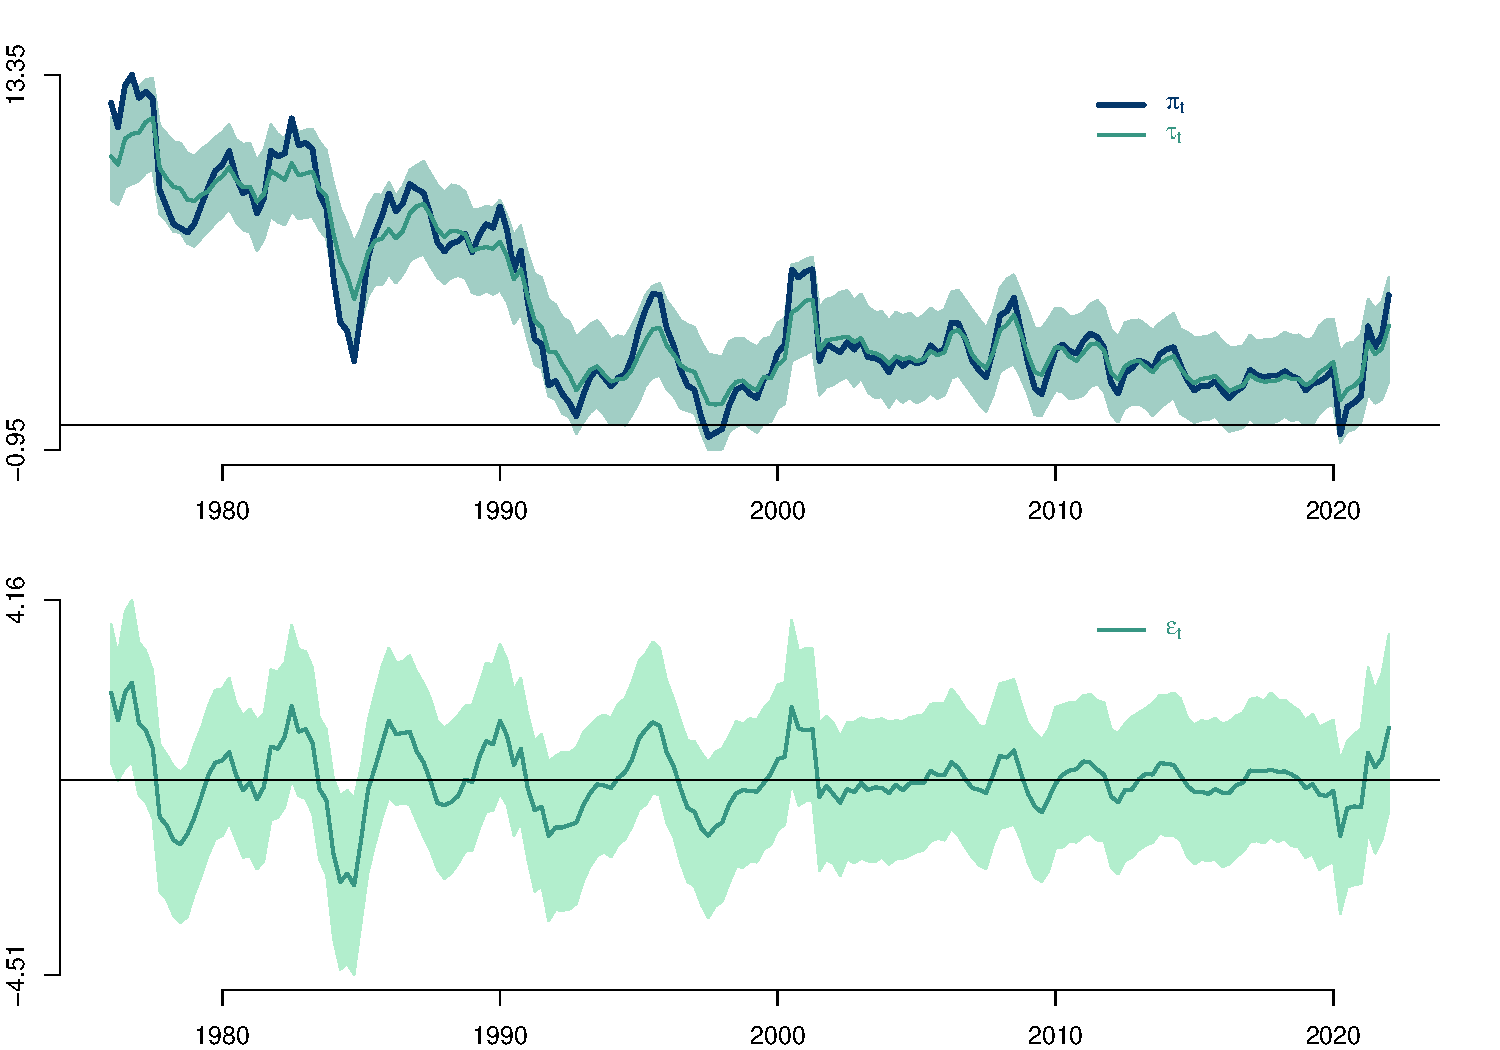
\includegraphics[scale=0.4, trim=2cm 0.5cm 2cm 0cm]{results/pi-rho-uc-ar4.pdf}

\end{frame}





\begin{frame}{Australian CPI inflation}

\bigskip\textbf{UC-AR(p) with gamma prior.}
\begin{align*}
y_t &= \tau_t + \epsilon_t\\[1ex]
\tau_t &= \mu + \tau_{t-1} + \eta_t\\[1ex]
\epsilon_t &= \alpha_1\epsilon_{t-1} + \dots + \alpha_p\epsilon_{t-p} +  e_t\\[2ex]
\begin{bmatrix}\eta_t \\ e_t\end{bmatrix}&\bigg|Y_{t-1} \sim ii\mathcal{N}\left(\mathbf{0}_2, \begin{bmatrix}\sigma_\eta^2 & 0 \\  & \sigma_e^2\end{bmatrix} \right)\\[2ex]
\sigma_\eta^2 &\mid\underline{s} \sim\mathcal{G}(s,a)
\end{align*}

\end{frame}





\begin{frame}{Australian CPI inflation}

\small
\begin{adjustwidth}{-0.5cm}{0cm}
\begin{center}
\textbf{Estimation results from UC-AR(p) models:} {\color{mcxs2}$\pi_t$ 1976Q1--2022Q1}

\footnotesize\smallskip\begin{tabular}{cccccccc}
\toprule
$\alpha_1$ & $\alpha_2$ & $\alpha_3$ & $\alpha_4$ & $\alpha_5$& \% s  & $\mu$ & $\sigma^2_\eta / \sigma^2_e$\\
\midrule
0.841 & 0.160 & 0.091 & -0.387 &  & 100 & -0.021 & 0.780 \\ 
 0.114 & 0.135 & 0.136 & 0.120 &  &  & 0.041 &  \\ [1ex]
\bottomrule
\end{tabular}

\smallskip 
\% s -- fraction of posterior draws for which stationarity condition holds\\
$\sigma^2_\eta / \sigma^2_e$ -- signal-to-noise ratio
\end{center}
\end{adjustwidth}
\end{frame}





\begin{frame}{Australian CPI inflation}

\small
\centering
\smallskip\textbf{Estimated trend and cycle from UC-AR(4) with gamma prior}

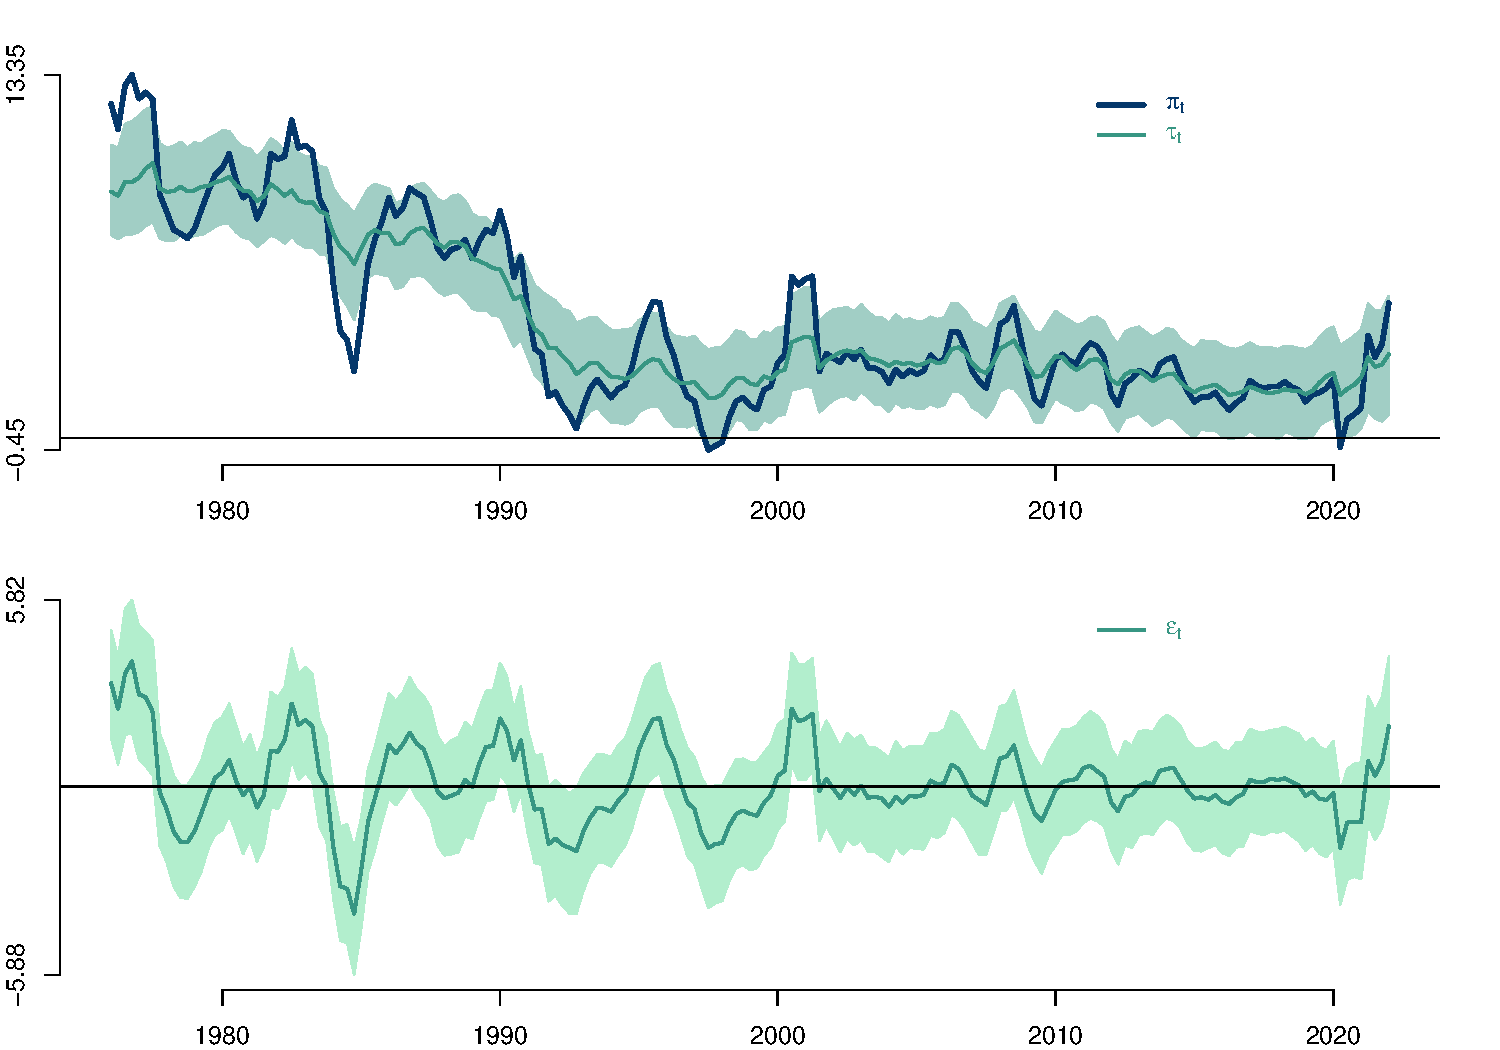
\includegraphics[scale=0.4, trim=2cm 0.5cm 2cm 0cm]{results/pi-gamma-uc-ar4.pdf}

\end{frame}





\begin{frame}{Australian CPI inflation}

\smallskip\textbf{Stochastic or deterministic trend?}

\smallskip {\color{mcxs2}Testing restriction} $\sigma^2_\eta=0$ {\color{mcxs2}is difficult. However}

$$
\sigma^2_\eta\mid\underline{s} \sim\mathcal{G}\left(2\underline{s}, \frac{1}{2}\right) \qquad\Rightarrow\qquad
\pm\sqrt{\sigma^2_\eta}\mid\underline{s} \sim\mathcal{N}\left(0, \underline{s}\right) 
$$

{\color{mcxs2}Testing restriction} $\pm\sqrt{\sigma^2_\eta}=0$ {\color{mcxs2}seems easier.}

\bigskip\textbf{Savage-Dickey density ratio for $\pm\sqrt{\sigma^2_\eta}=0$:}
$$
\frac{p\left(\pm\sqrt{\sigma^2_\eta}=0\mid data\right)}{p\left(\pm\sqrt{\sigma^2_\eta}=0\right)} = \frac{\Pr\left[\pm\sqrt{\sigma^2_\eta}=0\mid data\right]}{\Pr\left[\pm\sqrt{\sigma^2_\eta}=0\right]}
$$

\end{frame}


\begin{frame}{Australian CPI inflation}

\smallskip\textbf{Stochastic or deterministic trend?}
\centering
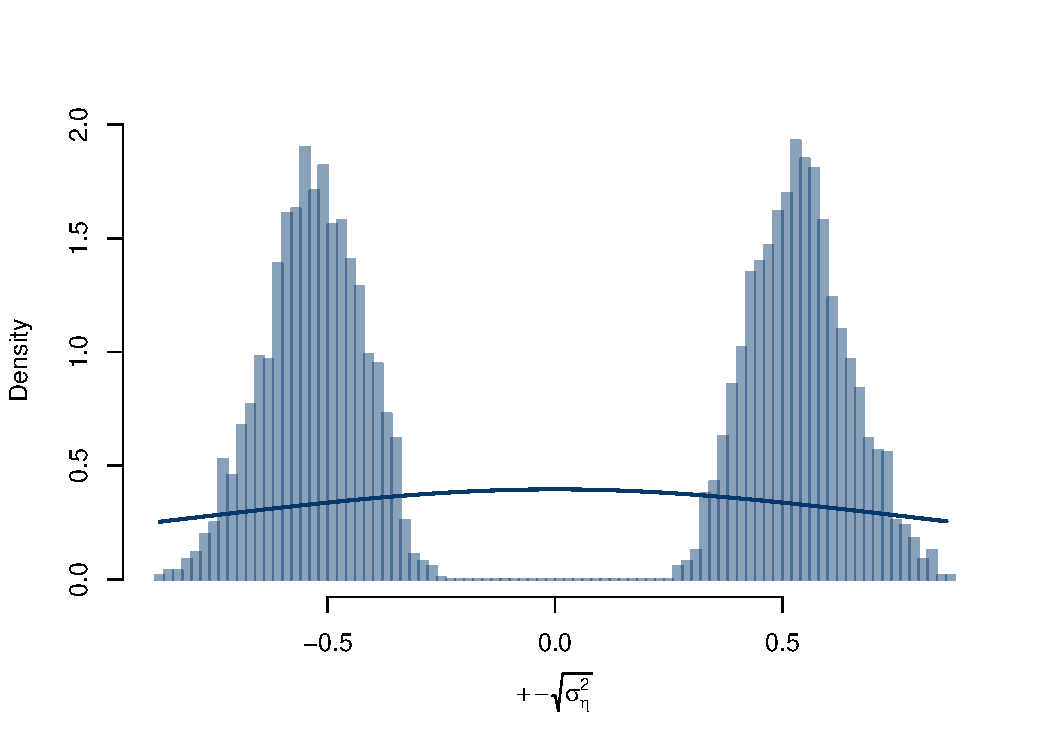
\includegraphics[scale=0.5, trim=2cm 0.5cm 2cm 1cm]{results/pi-gamma-omega.pdf}

{\color{mcxs2}The value of the SDDR is clearly less than 1 which constitutes strong Bayesian evidence against the restriction.}
\end{frame}







{\setbeamercolor{background canvas}{bg=mcxs5}
\begin{frame}

\begin{adjustwidth}{-0.5cm}{0cm}
\vspace{8.3cm}\Large
\textbf{{\color{mcxs3}UC model for} {\color{mcxs1}Australian CPI prices}}
\end{adjustwidth}

\end{frame}
}






\begin{frame}{Australian CPI prices}

\bigskip\textbf{UC-AR(4) with time-varying drift.}
\begin{align*}
y_t &= \tau_t + \epsilon_t\\[1ex]
\tau_t &= \mu_t + \tau_{t-1} + \eta_t\\[1ex]
\mu_t &= \mu_{t-1} + m_t\\[1ex]
\epsilon_t &= \alpha_1\epsilon_{t-1} + \dots + \alpha_4\epsilon_{t-4} +  e_t\\[2ex]
\begin{bmatrix}\eta_t \\ e_t\\ m_t\end{bmatrix}&\bigg|Y_{t-1} \sim ii\mathcal{N}\left(\mathbf{0}_3, \begin{bmatrix}\sigma_\eta^2 & 0 & 0 \\  & \sigma_e^2 &0 \\
&&\sigma_m^2\end{bmatrix} \right)
\end{align*}

\end{frame}



\begin{frame}{Australian CPI prices}

\begin{adjustwidth}{-0.5cm}{0cm}
\begin{center}
\textbf{Estimation results from UC-AR(4)} {\color{mcxs2}$cpi_t$ 1976Q1--2022Q1}

\small\smallskip\begin{tabular}{cccccccc}
\toprule
$\alpha_1$ & $\alpha_2$ & $\alpha_3$ & $\alpha_4$& \% s  & $\sigma^2_\eta / \sigma^2_e$& $\tau_0$ & $\mu_0$\\[1ex]
 0.211& -0.085&  0.017&  0.129&  0.956&  1.911&  2.816&  0.034\\
0.334& 0.222& 0.206& 0.188&    &    & 0.016& 0.024\\
\bottomrule
\end{tabular}

\smallskip 
\% s -- fraction of posterior draws for which stationarity condition holds\\
$\sigma^2_\eta / \sigma^2_e$ -- signal-to-noise ratio
\end{center}
\end{adjustwidth}
\end{frame}






\begin{frame}{Australian CPI prices}

\centering
\smallskip\textbf{Estimated trend.}

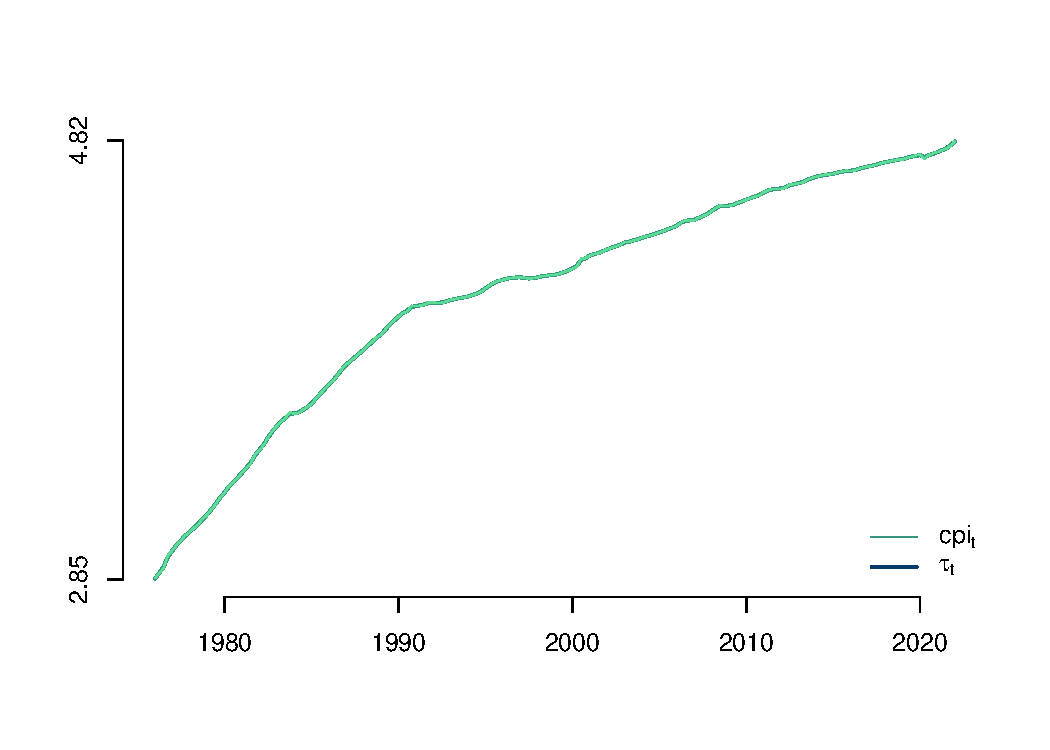
\includegraphics[scale=0.65, trim=2cm 0.5cm 2cm 2cm]{results/cpi-uc-tvpdrift-tau.pdf}

\end{frame}




\begin{frame}{Australian CPI prices}

\centering
\smallskip\textbf{Estimated quarterly inflation trend}

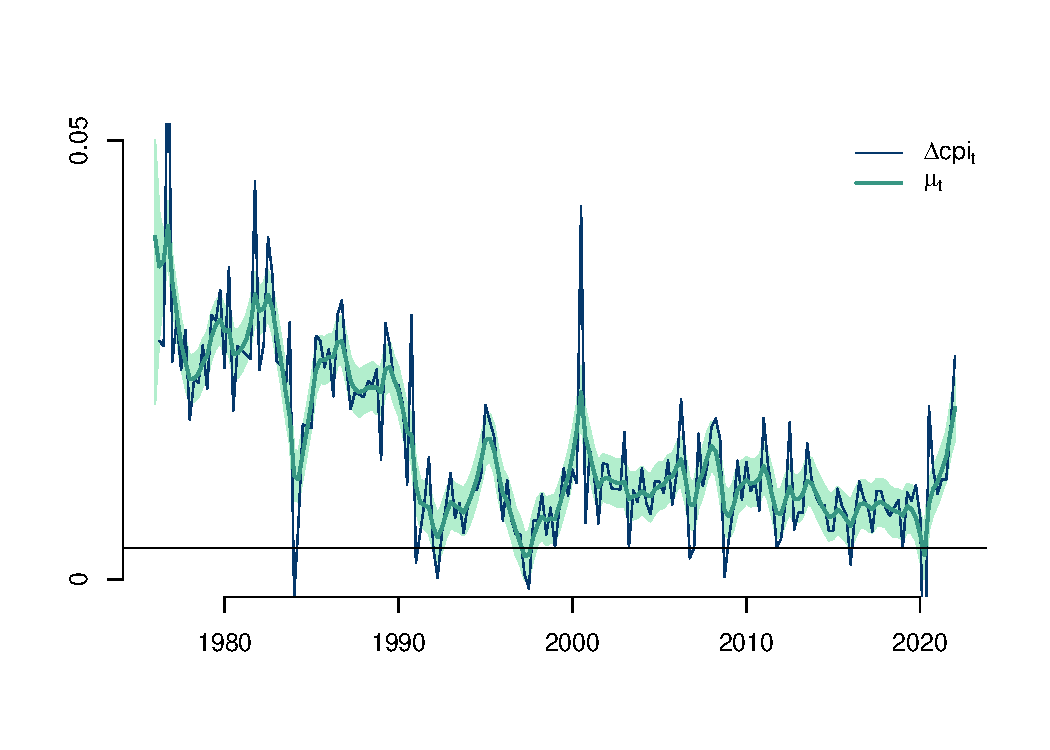
\includegraphics[scale=0.65, trim=2cm 0.5cm 2cm 2cm]{results/cpi-uc-tvpdrift-mu.pdf}

\end{frame}



\begin{frame}{Australian CPI prices}

\centering
\smallskip\textbf{Estimated cycle.}

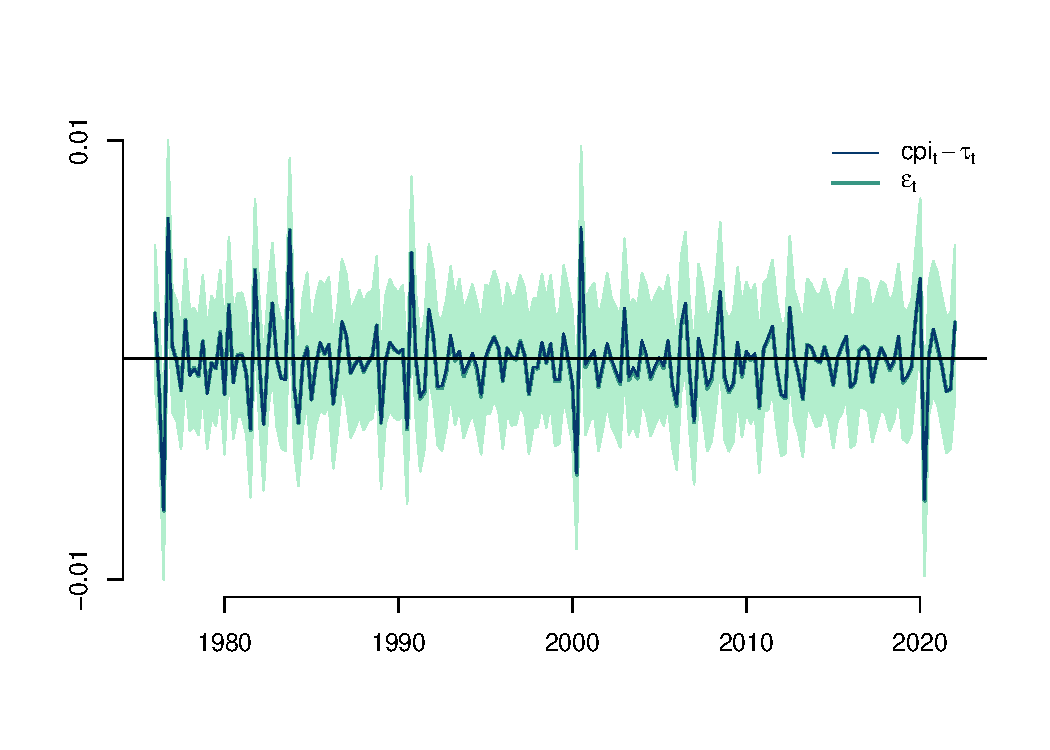
\includegraphics[scale=0.65, trim=2cm 0.5cm 2cm 2cm]{results/cpi-uc-tvpdrift-epsilon.pdf}

\end{frame}











{\setbeamercolor{background canvas}{bg=mcxs5}
\begin{frame}

\begin{adjustwidth}{-0.5cm}{0cm}
\vspace{8.3cm}\Large
\textbf{{\color{mcxs3}UC model for} {\color{mcxs1}Australian Real GDP}}
\end{adjustwidth}

\end{frame}
}






\begin{frame}{Australian real GDP}

\centering
\includegraphics[scale=0.55, trim=2cm 1cm 2cm 0cm]{results/data-gdp.pdf}

\bigskip\small{\color{mcxs2}
Quarterly data from 1959Q3 to 2021Q4 ($T=250$)\\ 
Downloaded from the ABS using }\\ \texttt{readabs::read\_abs(series\_id = "A2304402X")}

\end{frame}




\begin{frame}{Australian real GDP}

\centering
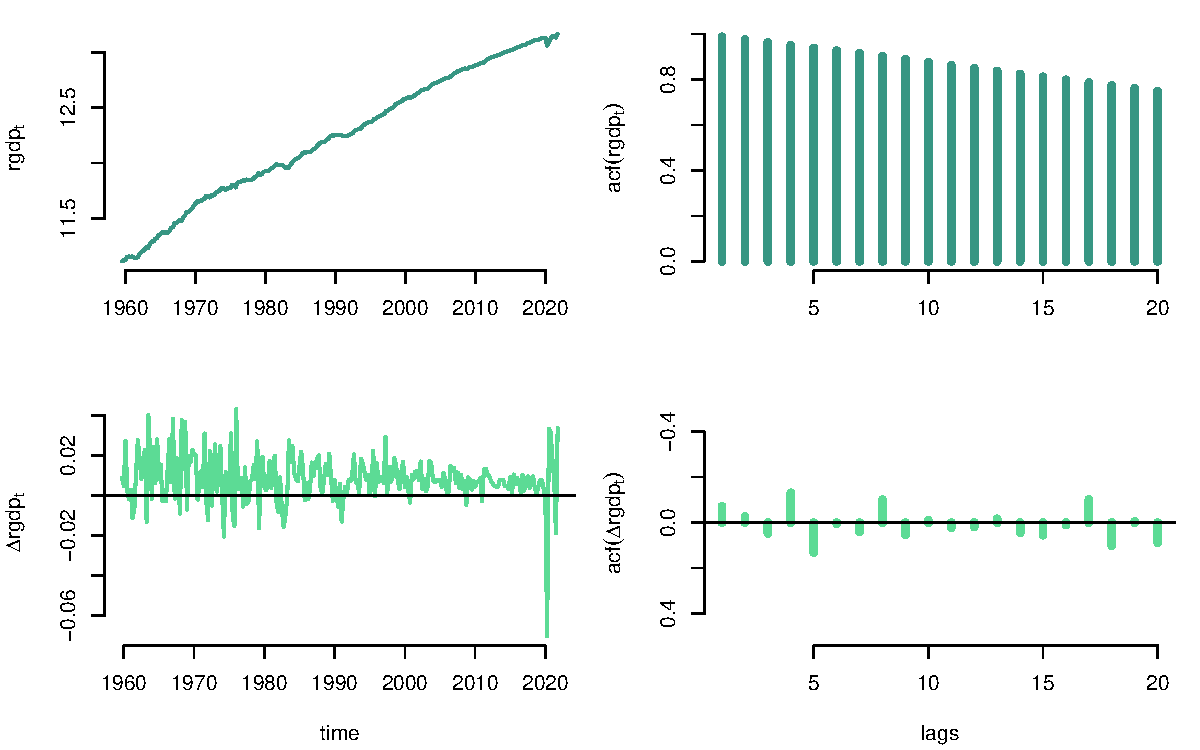
\includegraphics[scale=0.55, trim=2cm 0.5cm 2cm 0cm]{results/data-gdp-acf.pdf}

\bigskip\small{\color{mcxs2}
$rgdp_t= log(GDP_t)$ and $\Delta rgdp_t= rgdp_t - rgdp_{t-1}$ \\
Quarterly data from 1959Q3 to 2021Q4 ($T=250$)}

\end{frame}









\begin{frame}{Australian real GDP}

\bigskip\textbf{UC-AR(4) with time-varying drift.}
\begin{align*}
y_t &= \tau_t + \epsilon_t\\[1ex]
\tau_t &= \mu_t + \tau_{t-1} + \eta_t\\[1ex]
\mu_t &= \mu_{t-1} + m_t\\[1ex]
\epsilon_t &= \alpha_1\epsilon_{t-1} + \dots + \alpha_4\epsilon_{t-4} +  e_t\\[2ex]
\begin{bmatrix}\eta_t \\ e_t\\ m_t\end{bmatrix}&\bigg|Y_{t-1} \sim ii\mathcal{N}\left(\mathbf{0}_3, \begin{bmatrix}\sigma_\eta^2 & 0 & 0 \\  & \sigma_e^2 &0 \\
&&\sigma_m^2\end{bmatrix} \right)
\end{align*}

\end{frame}



\begin{frame}{Australian real GDP}

\begin{adjustwidth}{-0.5cm}{0cm}
\begin{center}
\textbf{Estimation results from UC-AR(4)} {\color{mcxs2}$gdp_t$ 1959Q3--2022Q1}

\small\smallskip\begin{tabular}{cccccccc}
\toprule
$\alpha_1$ & $\alpha_2$ & $\alpha_3$ & $\alpha_4$& \% s  & $\sigma^2_\eta / \sigma^2_e$& $\tau_0$ & $\mu_0$\\[1ex]
 0.007& -0.262& -0.149& -0.297&  0.992&  1.311& 11.072&  0.046\\
0.281& 0.208& 0.191& 0.141&    &    & 0.023& 0.031\\[1ex]
\bottomrule
\end{tabular}

\smallskip 
\% s -- fraction of posterior draws for which stationarity condition holds\\
$\sigma^2_\eta / \sigma^2_e$ -- signal-to-noise ratio
\end{center}
\end{adjustwidth}
\end{frame}






\begin{frame}{Australian real GDP}

\centering
\smallskip\textbf{Estimated trend.}

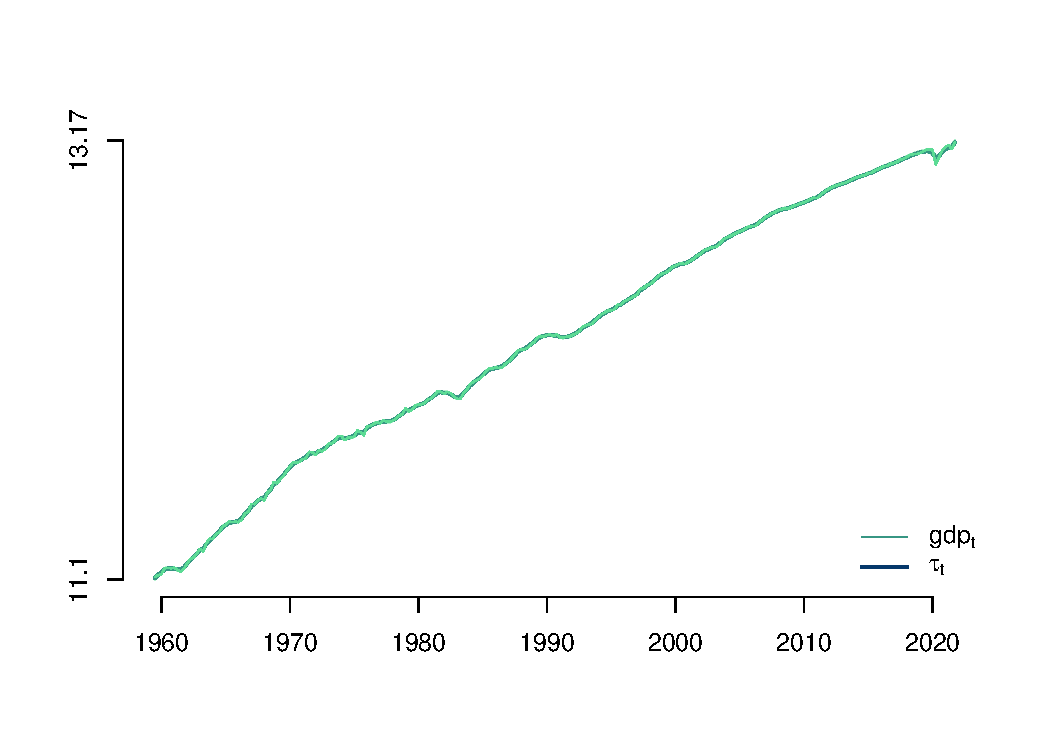
\includegraphics[scale=0.65, trim=2cm 0.5cm 2cm 2cm]{results/gdp-uc-tvpdrift-tau.pdf}

\end{frame}




\begin{frame}{Australian real GDP}

\centering
\smallskip\textbf{Estimated output gap.}

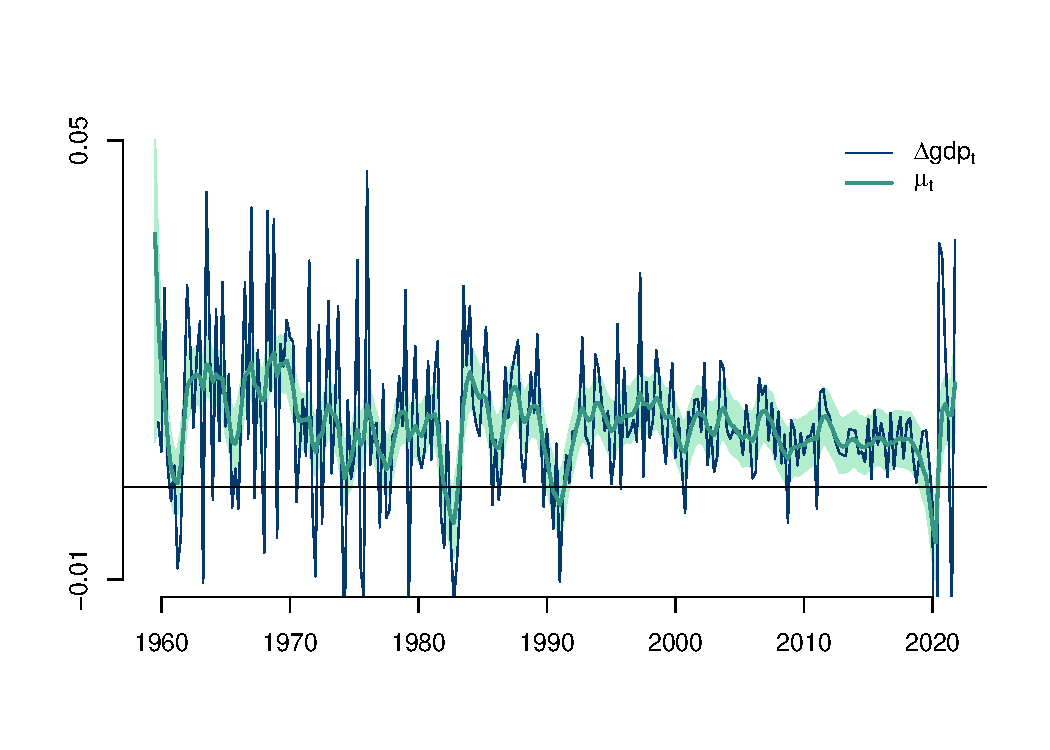
\includegraphics[scale=0.65, trim=2cm 0.5cm 2cm 2cm]{results/gdp-uc-tvpdrift-mu.pdf}

\end{frame}



\begin{frame}{Australian real GDP}

\centering
\smallskip\textbf{Estimated residuals.}

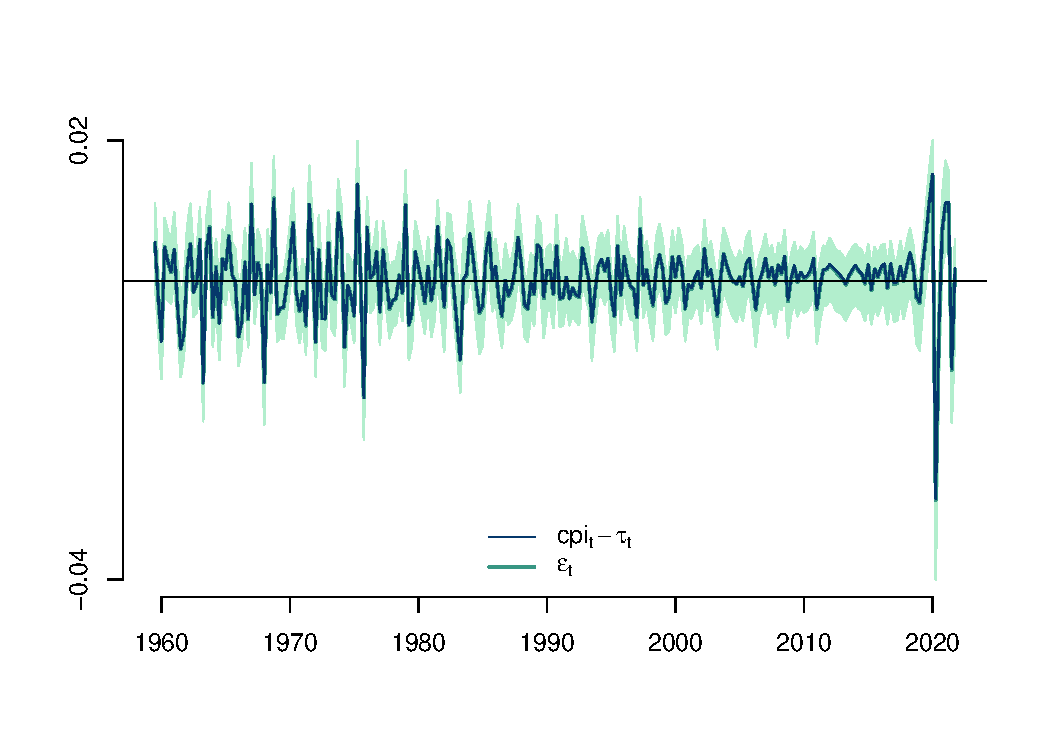
\includegraphics[scale=0.65, trim=2cm 0.5cm 2cm 2cm]{results/gdp-uc-tvpdrift-epsilon.pdf}

\end{frame}















{\setbeamercolor{background canvas}{bg=mcxs5}
\begin{frame}{Australian CPI prices and inflation}

\bigskip\textbf{Unobserved Component} models correctly capture the dynamics in Australian CPI prices and inflation.

\bigskip\textbf{Trend-cycle decomposition} indicates increasing long-run inflation trend.

\bigskip\textbf{Hierarchical priors} are the essential extension.

\end{frame}
}




\end{document} 